\section{Нейтринная томография Земли}
\label{sec:tomography}
В этом разделе рассматривается возможность уточнения распределения плотности Земли с помощью нейтрино сверхвысоких энергий.  
В настоящее время сведения о внутренней структуре и плотности Земли получены главным образом из сейсмологических наблюдений, в частности в рамках модели PREM (Preliminary Reference Earth Model)~\cite{dziewonskiPREM1981}.

Идея использовать нейтринные осцилляции при энергиях порядка нескольких ГэВ для реконструкции плотности Земли активно обсуждается в контексте современных нейтринных детекторов, таких как DUNE, ORCA и PINGU~\cite{winterTomography2013,akhmedovTomography2006}.  
Однако такой подход сталкивается с серьёзными экспериментальными трудностями: требуется (i) высокая точность реконструкции энергии, (ii)направления приходящих нейтрино, (iii) большая масса детектора, (iv) эффективное подавление фоновых событий. Все эти требования  довольно сложно удовлетворить практически для ГэВ-ных энергий нейтрино.

Альтернативный метод основан на эффекте поглощения нейтрино сверхвысоких энергий ($E_\nu \gtrsim 10$~ТэВ) при прохождении через Землю~\cite{gandhiAbsorption1998,franceTomography2019}.  
Поскольку сечение взаимодействия нейтрино растёт с энергией, поток таких частиц существенно ослабляется, особенно для траекторий, проходящих через ядро.  
Однако чувствительность этого метода, основанного только на поглощении (заряжённый ток), ограничена быстрым спадом числа наблюдаемых событий при росте энергии нейтрино.

В настоящей работе показано, что учёт \emph{регенерации потока} за счёт взаимодействий по нейтральному току существенно повышает чувствительность томографического метода.  
Нейтральные токи возвращают часть потока нейтрино на меньшие энергии, обеспечивая статистически значимое число событий даже при $E_\nu \gtrsim 1$~ПэВ.  
Таким образом, регенерация делает нейтринную томографию Земли практически осуществимой с использованием будущих крупномасштабных детекторов, таких как IceCube-Gen2 и KM3NeT.

\subsection{Важность регенерации}

При прохождении нейтрино сквозь Землю поток ослабляется вследствие взаимодействий по заряженному и нейтральному току.  
Заряжённый ток (\textit{CC}) отвечает за поглощение нейтрино: каждая реакция
\[
\nu_\ell + N \to \ell + X
\]
полностью удаляет нейтрино из пучка, и поток убывает экспоненциально:
\[
F_\nu(X(\theta_d),E_\nu) \propto 
e^{-N_A\,\sigma_{CC}(E)\,X(\theta_d)}, 
\qquad
X(\theta_d) = \int \rho(\ell)\, d\ell .
\]
Это создаёт базовую чувствительность к плотности Земли, однако число событий при этом быстро уменьшается с ростом энергии, и общая эффективность метода, основанного только на заряжённом токе, остаётся невысокой.

Нейтральный ток (\textit{NC}), напротив, не уничтожает нейтрино, а лишь понижает его энергию:
\[
\nu_\ell + N \to \nu_\ell' + X.
\]
Благодаря этому часть потока, потерянная на высоких энергиях, регенерируется на меньших энергиях, что приводит к заметному росту числа событий в детекторе.

Учёт \emph{регенерации нейтрино по нейтральному току} существенно повышает чувствительность нейтринной томографии Земли: без него поток нейтрино экспоненциально затухает, тогда как включение этого эффекта позволяет сохранять измеримый сигнал даже при $E_\nu \gtrsim 1$~ПэВ. 
Хотя влияние нейтрального тока на спектр нейтрино отмечалось и ранее, в настоящей работе этот эффект впервые детально рассмотрен с точки зрения его вклада в чувствительность методов томографии.

На рис.~\ref{EF1} показано, что вклад нейтрального тока становится доминирующим для нейтрино, проходящих через ядро Земли.

\begin{figure}[!h]
\centering
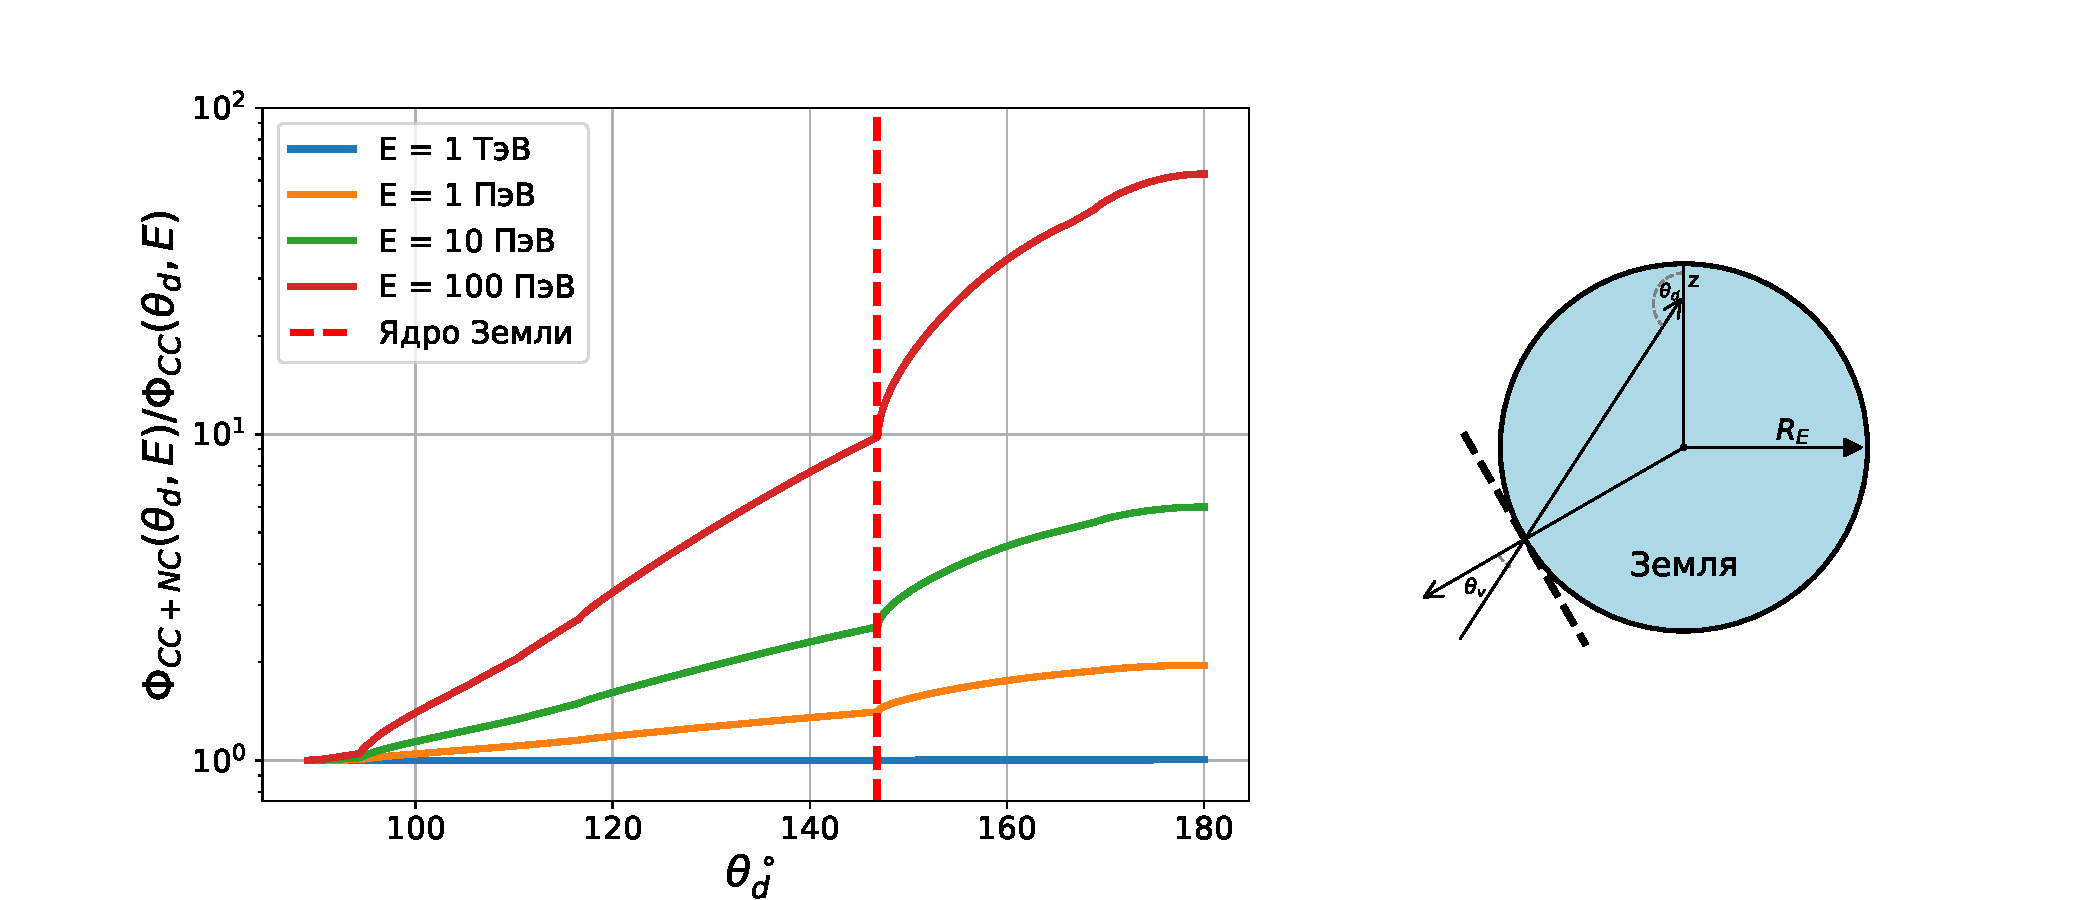
\includegraphics[width=\linewidth]{images/NuProp/rhh12zf_flux_index_CT18ZNNLO.pdf}
\caption{Влияние нейтрального тока на поток нейтрино в детекторе в зависимости от угла прихода $\theta_d$ и энергии $E_\nu$.  
Учёт нейтрального тока существенно увеличивает число регенерированных нейтрино, особенно для траекторий, проходящих через ядро Земли.}
\label{EF1}
\end{figure}

Таким образом, измеряя энергетические спектры нейтрино, прошедших через Землю, можно реконструировать распределение плотности вещества вдоль их траекторий — вплоть до ядра планеты.



% \subsection{Поглощение за счет нейтрального и заряженного токов}
% В конце зададимся вопросом, как изменяется показатель потока при прохождении нейтрино сквозь Землю за счёт разных взаимодействий. Предположим, что начальный и конечный потоки имеют форму 
% \begin{equation}
%     F_{in/fin}(E) = \Phi_0 E^{-\gamma_{in/fin}(E)}.
% \end{equation}
% На рис. (\ref{EF3}) можно видеть, что показатель потока начинает сильно изменяться при энергиях выше 10 ТэВ. Таким образом, для нейтрино высоких энергий, проходящих сквозь Землю, спектр будет сильно изменяться, поэтому количество событий для таких нейтрино будет сильно меньше ожидаемых. Нейтрино же, летящие сверху, не подвергнутся такому подавлению потока.    
% \begin{figure}[!h]
% \centering
% 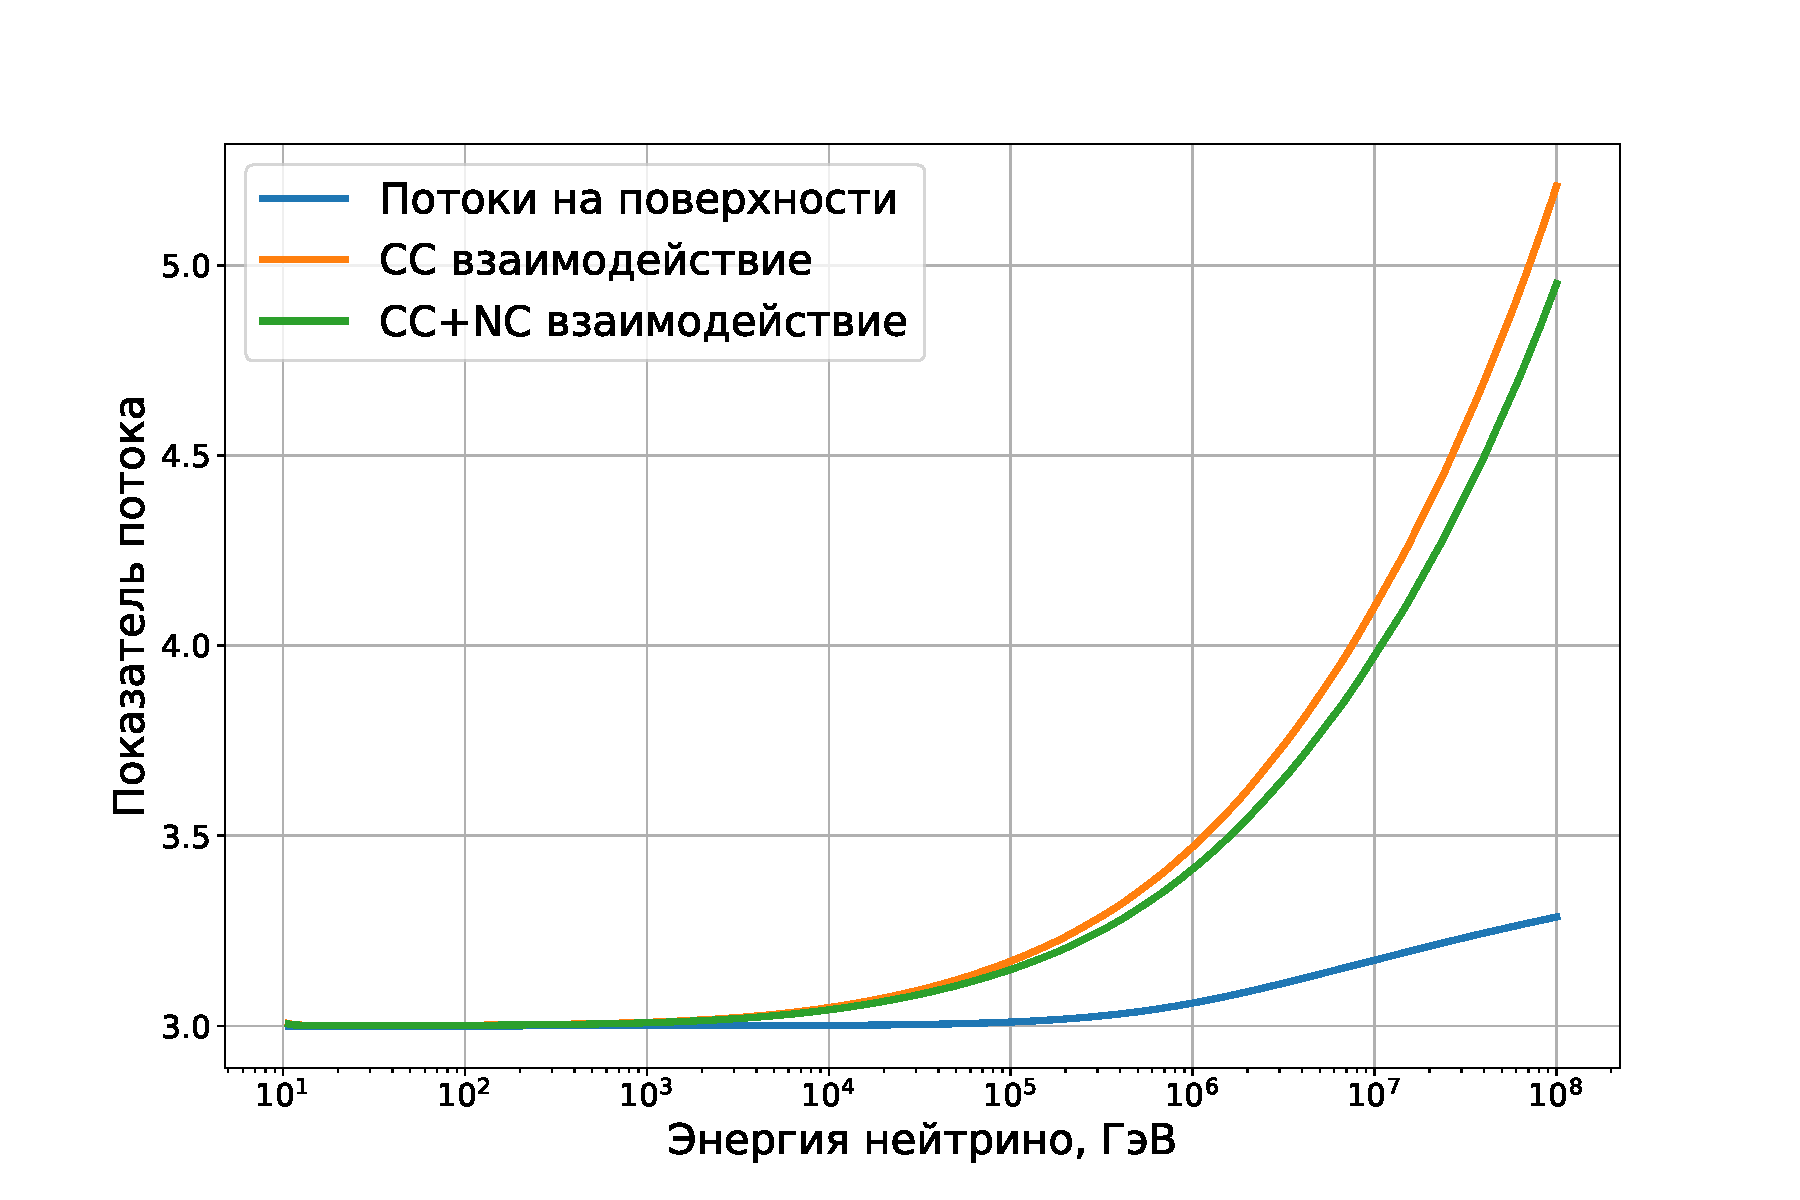
\includegraphics[width=1.1\linewidth]{images/NuProp/rzf_flux_index_CT18ZNNLO.pdf}
% \caption{Изменение показателя потока нейтрино для пучка, проходящего сквозь Землю в зависимости от энергии при учете разных типов взаимодействия.}
% \label{EF3}
% \end{figure}

\subsection{Статистический анализ}

Для количественной оценки чувствительности нейтринной томографии рассмотрим две гипотезы:  
\begin{itemize}
  \item $H_0$ — стандартная модель плотности Земли, соответствующая модели PREM~\cite{dziewonskiPREM1981};
  \item $H_1$ — альтернативные модели, описывающие возможные отклонения от PREM.
\end{itemize}

В качестве альтернативных гипотез рассматриваются три варианты распределения плотности:  
(1) модель с усреднённым ядром,  
(2) модель с линейным градиентом плотности в ядре,  
(3) модель с усреднёнными мантией и ядром.  

Гипотезы (2) и (3) рассматриваются в приложении~\ref{sec:appTomography}.

Сравнение гипотез проводится по статистике $\chi^2$, определяемой как
\begin{equation}
\label{eq:chi2_def}
\Delta\chi^2 = 2\sum_{i,j}
\left[
  N_{ij}^{(0)} - N_{ij}^{(1)} 
  + N_{ij}^{(1)}\ln\!\left(\frac{N_{ij}^{(1)}}{N_{ij}^{(0)}}\right)
\right],
\end{equation}
где $N^{(k)}_{ij}$ — ожидаемое число событий в интервале по энергии и углу для гипотезы $H_k$.  
Такое определение эквивалентно логарифму отношения правдоподобий (LLR) в предположении пуассоновской статистики и используется, например, в анализах коллабораций IceCube и ANTARES.

Для оценки статистической мощности метода рассчитывались полные числа событий в нейтринном телескопе объёмом $1~\text{км}^3$ за один год наблюдений при разных моделях плотности. На основе значений $\Delta\chi^2$ проверяется гипотеза $H_0$: большие значения статистики указывают на отличие рассматриваемой модели $H_1$ от PREM.

Для последующего анализа в качестве астрофизических потоков возьмем фит для диффузионного потока, рассчитанного коллаборацией IceCube ~\cite{Abbasi_2024}. Данные потоки рассчитаны в предположении степенного спектра на 1 флейвор нейтрино. В качестве атмосферных нейтринных потоков взяты потоки, полученные командой С. И. Синеговского~\cite{sinegovskaya2015}, рассчитанных на 1 флейвор нейтрино. В дальнейшем весь анализ будет проведён с учетом только мюонного флейвора ($\nu_{\mu}$ + $\bar{\nu}_{\mu}$).
  \begin{figure}[!h]
    \centering
    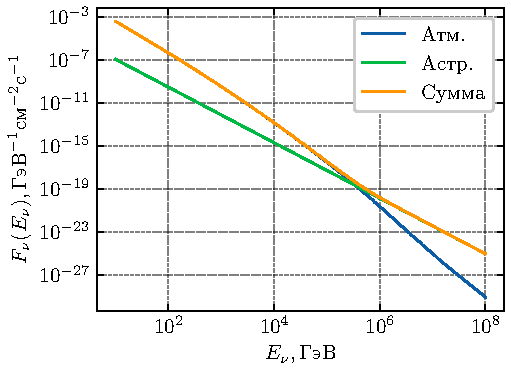
\includegraphics[width=0.8\linewidth]{images/NuProp/fluxes.pdf}
    \caption{Атмосферные и астрофизические нейтринные потоки для мюонного флейвора.}
    \label{NuFluxes_astro_and_atmo}
  \end{figure}
\subsection*{Усреднённое ядро и мантия.}  
В качестве альтернативной гипотезы $H_1$ используется модель с постоянной плотностью $\rho = 8.853~\text{г/см}^3$ в области внутреннего ядра, внешнего ядра и мантии (до радиуса $5600~\text{км}$).  
В остальной части модель совпадает с PREM.  
Для данной пары гипотез ($H_0$, $H_1$) получено значение $\Delta\chi^2 = 6.84$, что соответствует статистической значимости $2.62\sigma$ при одном числе степеней свободы.
  
  \begin{figure}[!h]
    \centering
    \includegraphics[width=0.8\linewidth]{images/NuProp/chi2_rzf_2dxsCT10nlo_PREM_vs_PREM_man_and_ker.png}
    \caption{Распределение статистики $\Delta\chi^2$, полученной при сравнении чисел нейтринных событий для гипотез $H_0$ (модель PREM) и $H_1$ (усреднённые ядро и мантия).}
    \label{NuTom1}
  \end{figure}

Из анализа распределения $\Delta\chi^2$ на рис.~(\ref{NuTom1}) следует, что наибольшая чувствительность нейтринной томографии приходится на диапазон энергий  
\[
E_\nu \sim 10^2\text{–}10^6~\text{ГэВ},
\]
где сечения взаимодействий уже достаточно велики для заметного ослабления потока, но интенсивность ещё не слишком мала.  
Максимум чувствительности наблюдается около $E_\nu \sim 10^4~\text{ГэВ}$.  
Зависимость по углу прихода нейтрино определяется характером альтернативной модели: при изменении плотности в мантии максимум по углу смещается к меньшим значениям $\theta_d$, что отражает различие в эффективных толщинах вещества вдоль траекторий.
